\section{Resolução do Desafio}

\begin{minipage}{\linewidth}
  \centering
  \begin{minipage}{0.45\linewidth}
    Dado o circuito da \textbf{Figura \ref{fig:resCircuitoDesafio}},
    considerar: $R_1 = 330\Omega$,
                $R_2 = 150\Omega$,
                $R_3 = 270\Omega$, \\
                $R_4 = 400\Omega$,
                $R_5 = 100\Omega$ e
                $V_{CC} = 10V$.
    \begin{itemize}
      \item Calcular a intensidade da corrente em cada resistor;
      \item Calcular a queda de tensão em cada resistor;
    \end{itemize}
  \end{minipage}
  \hspace{0.05\linewidth}
  \begin{minipage}{0.45\linewidth}
    \begin{figure}[H]
      \centering
      \caption{Circuito elétrico misto}
      \label{fig:resCircuitoDesafio}
      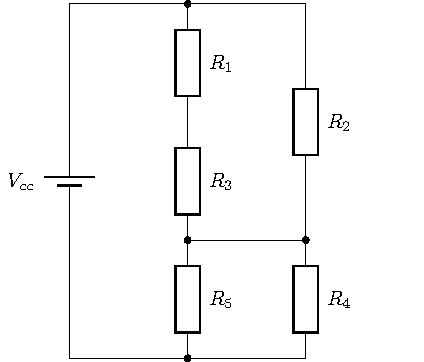
\includegraphics[scale=1.0]{fig-desafio}

      {\small Fonte: Próprio autor.}
    \end{figure}
  \end{minipage}
\end{minipage}






\subsection{Passo 1: Identificação dos nós}

\begin{minipage}{\linewidth}
  \centering
  \begin{minipage}{0.45\linewidth}
    Dados do circuito: \\
                $R_1 = 330\Omega$,
                $R_2 = 150\Omega$,
                $R_3 = 270\Omega$, \\
                $R_4 = 400\Omega$ e
                $R_5 = 100\Omega$.
  \end{minipage}
  \hspace{0.05\linewidth}
  \begin{minipage}{0.45\linewidth}
    \begin{figure}[H]
      \centering
      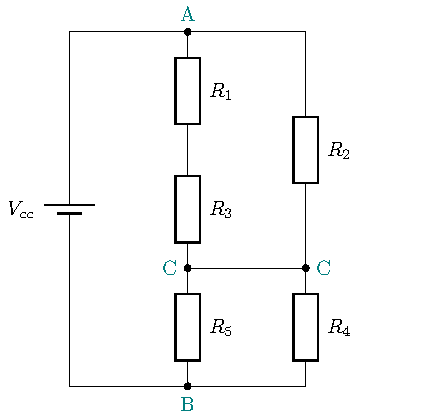
\includegraphics[scale=1.0]{fig-desafioPasso1}
    \end{figure}
  \end{minipage}
\end{minipage}










\subsection{Passo 2: Identificação de resistores em série}

\begin{minipage}{\linewidth}
  \centering
  \begin{minipage}{0.45\linewidth}
    Dados do circuito: \\
                $R_1 = 330\Omega$,
                $R_2 = 150\Omega$,
                $R_3 = 270\Omega$, \\
                $R_4 = 400\Omega$ e
                $R_5 = 100\Omega$.

      \begin{eqnarray}
        R_A & = & R_1 + R_3 \nonumber\\
        R_A & = & 330 + 270 \nonumber\\
        R_A & = & 600\Omega \nonumber
      \end{eqnarray}

  \end{minipage}
  \hspace{0.05\linewidth}
  \begin{minipage}{0.45\linewidth}
    \begin{figure}[H]
      \centering
      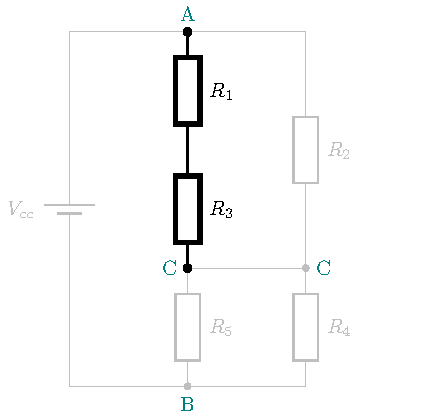
\includegraphics[scale=1.0]{fig-desafioPasso2}
    \end{figure}
  \end{minipage}
\end{minipage}







\subsection{Passo 3: Identificação de resistores em paralelo}

\begin{minipage}{\linewidth}
  \centering
  \begin{minipage}{0.45\linewidth}
    Dados do circuito: \\
                $R_1 = 330\Omega$,
                $R_2 = 150\Omega$,
                $R_3 = 270\Omega$, \\
                $R_4 = 400\Omega$ e
                $R_5 = 100\Omega$,\\
                $R_A = R_1 + R_3 = 600\Omega$.
       \begin{eqnarray}
         G_B & = & G_A + G_2 \nonumber\\
         R_B & = & R_A // R_2 \nonumber\\
         R_B & = & \frac{1}{\frac{1}{R_A} + \frac{1}{R_2} } \nonumber\\
         R_B & = & \frac{1}{\frac{1}{600} + \frac{1}{150} } \nonumber\\
         R_B & = & 120\Omega \nonumber
       \end{eqnarray}

  \end{minipage}
  \hspace{0.05\linewidth}
  \begin{minipage}{0.45\linewidth}
    \begin{figure}[H]
      \centering
      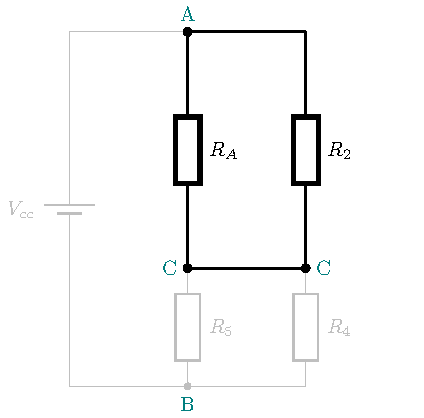
\includegraphics[scale=1.0]{fig-desafioPasso3}
    \end{figure}
  \end{minipage}
\end{minipage}








\subsection{Passo 4: Identificação de resistores em paralelo}

\begin{minipage}{\linewidth}
  \centering
  \begin{minipage}{0.45\linewidth}
    Dados do circuito: \\
                $R_1 = 330\Omega$,
                $R_2 = 150\Omega$,
                $R_3 = 270\Omega$, \\
                $R_4 = 400\Omega$ e
                $R_5 = 100\Omega$,\\
                $R_A = R_1 + R_3 = 600\Omega$, \\
                $R_B = R_A // R_2 = 120\Omega$.
        \begin{eqnarray}
         G_C & = & G_4 + G_5 \nonumber\\
         R_C & = & R_4 // R_5 \nonumber\\
         R_C & = & \frac{R_4 . R_5}{R_4 + R_5} \nonumber\\
         R_C & = & \frac{400 . 100}{400 + 100} \nonumber\\
         R_C & = & 80\Omega \nonumber
        \end{eqnarray}

  \end{minipage}
  \hspace{0.05\linewidth}
  \begin{minipage}{0.45\linewidth}
    \begin{figure}[H]
      \centering
      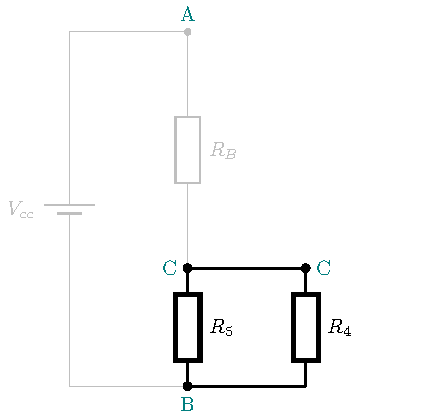
\includegraphics[scale=1.0]{fig-desafioPasso4}
    \end{figure}
  \end{minipage}
\end{minipage}






\subsection{Passo 5: Identificação de resistores em série}

\begin{minipage}{\linewidth}
  \centering
  \begin{minipage}{0.45\linewidth}
    Dados do circuito: \\
                $R_1 = 330\Omega$,
                $R_2 = 150\Omega$,
                $R_3 = 270\Omega$, \\
                $R_4 = 400\Omega$ e
                $R_5 = 100\Omega$,\\
                $R_A = R_1 + R_3 = 600\Omega$, \\
                $R_B = R_A // R_2 = 120\Omega$, \\
                $R_C = R_4 // R_5 = 80\Omega$.
        \begin{eqnarray}
          R_T & = & R_B + R_C \nonumber\\
          R_T & = & 120 + 80 \nonumber\\
          R_T & = & 200\Omega \nonumber
        \end{eqnarray}

  \end{minipage}
  \hspace{0.05\linewidth}
  \begin{minipage}{0.45\linewidth}
    \begin{figure}[H]
      \centering
      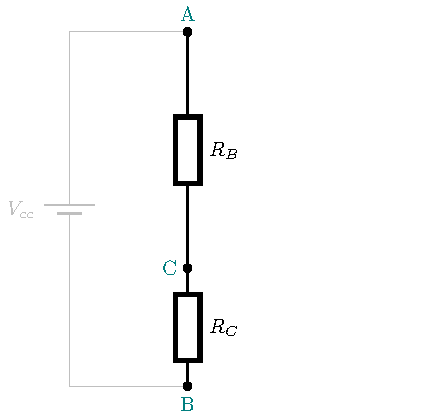
\includegraphics[scale=1.0]{fig-desafioPasso5}
    \end{figure}
  \end{minipage}
\end{minipage}



\subsection{Passo 6: Resistência Total do Circuito}

\begin{minipage}{\linewidth}
  \centering
  \begin{minipage}{0.45\linewidth}
    Dados do circuito: \\
                $R_1 = 330\Omega$,
                $R_2 = 150\Omega$,
                $R_3 = 270\Omega$, \\
                $R_4 = 400\Omega$ e
                $R_5 = 100\Omega$,\\
                $R_A = R_1 + R_3 = 600\Omega$, \\
                $R_B = R_A // R_2 = 120\Omega$, \\
                $R_C = R_4 // R_5 = 80\Omega$, \\
                $R_T = R_B + R_C = 200\Omega$.
  \end{minipage}
  \hspace{0.05\linewidth}
  \begin{minipage}{0.45\linewidth}
    \begin{figure}[H]
      \centering
      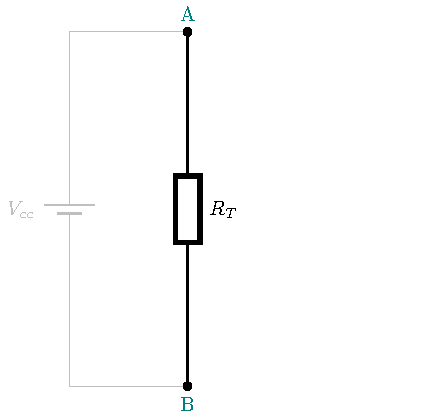
\includegraphics[scale=1.0]{fig-desafioPasso6}
    \end{figure}
  \end{minipage}
\end{minipage}





\subsection{Passo 7: Corrente total}

\begin{minipage}{\linewidth}
  \centering
  \begin{minipage}{0.45\linewidth}
    Dados do circuito: \\
                $R_1 = 330\Omega$,
                $R_2 = 150\Omega$,
                $R_3 = 270\Omega$, \\
                $R_4 = 400\Omega$ e
                $R_5 = 100\Omega$,\\
                $R_A = R_1 + R_3 = 600\Omega$, \\
                $R_B = R_A // R_2 = 120\Omega$, \\
                $R_C = R_4 // R_5 = 80\Omega$, \\
                $R_T = R_B + R_C = 200\Omega$.

                \begin{eqnarray}
                  V_{AB} & = & V_{CC} = 10 V \nonumber\\
                  \nonumber\\
                  I_T = \frac{V_{AB}}{R_T} & = & \frac{10}{200} = 0,05 A \nonumber
                \end{eqnarray}
  \end{minipage}
  \hspace{0.05\linewidth}
  \begin{minipage}{0.45\linewidth}
    \begin{figure}[H]
      \centering
      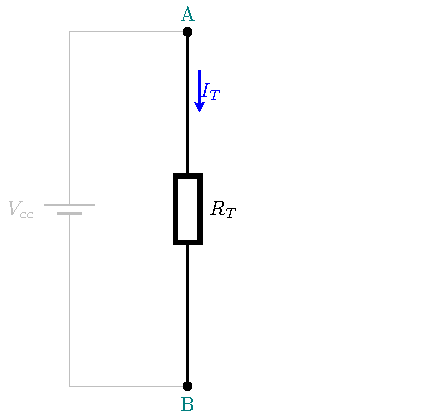
\includegraphics[scale=1.0]{fig-desafioPasso7}
    \end{figure}
  \end{minipage}
\end{minipage}





\subsection{Passo 8: Divisor de tensão}

\begin{minipage}{\linewidth}
  \centering
  \begin{minipage}{0.45\linewidth}
    Dados do circuito: \\
                $R_1 = 330\Omega$,
                $R_2 = 150\Omega$,
                $R_3 = 270\Omega$, \\
                $R_4 = 400\Omega$,
                $R_5 = 100\Omega$,
                $V_{CC} = 10V$, \\
                $R_A = R_1 + R_3 = 600\Omega$, \\
                $R_B = R_A // R_2 = 120\Omega$, \\
                $R_C = R_4 // R_5 = 80\Omega$, \\
                $R_T = R_B + R_C = 200\Omega$, \\
                \color{blue}{$I_T = \frac{V_{AB}}{R_T} = 0,05 A$}.
                \color{red}
    \begin{eqnarray}
      V_{R_B} = \frac{R_B}{R_T} . V_{AB} & = & \frac{120}{200} . 10 = 6V \nonumber\\
      \nonumber\\
      V_{R_C} = I_T.R_C & = & 0,05.80 = 4V
    \end{eqnarray}
  \end{minipage}
  \hspace{0.05\linewidth}
  \begin{minipage}{0.45\linewidth}
    \begin{figure}[H]
      \centering
      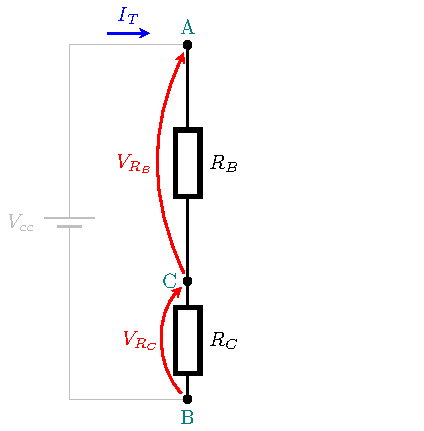
\includegraphics[scale=1.0]{fig-desafioPasso8}
    \end{figure}
  \end{minipage}
\end{minipage}





\subsection{Passo 9: Divisão da corrente}

\begin{minipage}{\linewidth}
  \centering
  \begin{minipage}{0.45\linewidth}
    Dados do circuito: \\
                $R_1 = 330\Omega$,
                $R_2 = 150\Omega$,
                $R_3 = 270\Omega$, \\
                $R_4 = 400\Omega$,
                $R_5 = 100\Omega$,
                $V_{CC} = 10V$, \\
                $R_A = R_1 + R_3 = 600\Omega$, \\
                $R_B = R_A // R_2 = 120\Omega$, \\
                $R_C = R_4 // R_5 = 80\Omega$, \\
                $R_T = R_B + R_C = 200\Omega$, \\
                \color{blue}{$I_T = \frac{V_{AB}}{R_T} = 0,05 A$},\\
                \color{red}{$V_{R_B} = \frac{R_B}{R_T} . V_{AB} = 6V$},\\
                \color{red}{$V_{R_C} = R_C.I_T = 4V$}.
    \begin{eqnarray}
      V_{R_C} = V_{CB} & = & V_{R_5} = V_{R_4} \nonumber
    \end{eqnarray}
    \color{blue}
    \vspace{-10mm}
    \begin{eqnarray}
      I_{R_5} = \frac{V_{R_5}}{R_5} & = & \frac{4}{100} = 0,04 A \nonumber\\
      \nonumber\\
      I_{R_4} = \frac{V_{R_4}}{R_4} & = & \frac{4}{400} = 0,01 A \nonumber
    \end{eqnarray}
  \end{minipage}
  \hspace{0.05\linewidth}
  \begin{minipage}{0.45\linewidth}
    \begin{figure}[H]
      \centering
      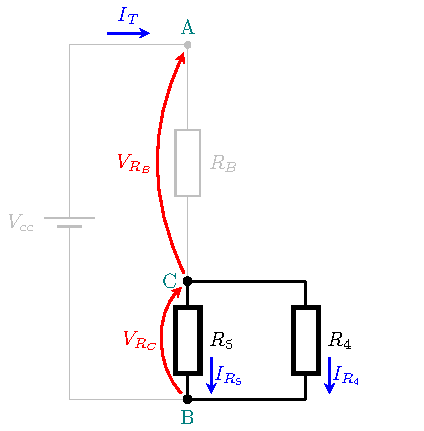
\includegraphics[scale=1.0]{fig-desafioPasso9}
    \end{figure}
  \end{minipage}
\end{minipage}








\subsection{Passo 10: Divisão da corrente}

\begin{minipage}{\linewidth}
  \centering
  \begin{minipage}{0.45\linewidth}
    Dados do circuito: \\
                $R_1 = 330\Omega$,
                $R_2 = 150\Omega$,
                $R_3 = 270\Omega$, \\
                $R_4 = 400\Omega$,
                $R_5 = 100\Omega$,
                $V_{CC} = 10V$, \\
                $R_A = R_1 + R_3 = 600\Omega$, \\
                $R_B = R_A // R_2 = 120\Omega$, \\
                $R_C = R_4 // R_5 = 80\Omega$, \\
                $R_T = R_B + R_C = 200\Omega$, \\
                \color{blue}
                $I_T = \frac{V_{AB}}{R_T} = 0,05 A$,\\
                \color{red}
                $V_{R_B} = \frac{R_B}{R_T} . V_{AB} = 6V$,\\
                $V_{R_C} = R_C.I_T = 4V$, \\
                $V_{R_C} = V_{CB} = V_{R_5} = V_{R_4}$,\\
                \color{blue}
                $I_{R_5} = V_{R_5} / R_5 = 0,04 A $, \\
                $I_{R_4} = V_{R_4} / R_4 = 0,01 A$.
    \color{red}
    \begin{eqnarray}
      V_{R_B} = V_{AC} & = & V_{R_A} = V_{R_2} \nonumber
    \end{eqnarray}
    \color{blue}
    \vspace{-10mm}
    \begin{eqnarray}
      I_{R_A} = \frac{V_{R_A}}{R_A} & = & \frac{6}{600} = 0,01 A \nonumber\\
      \nonumber\\
      I_{R_2} = \frac{V_{R_2}}{R_2} & = & \frac{6}{150} = 0,04 A \nonumber
    \end{eqnarray}
  \end{minipage}
  \hspace{0.05\linewidth}
  \begin{minipage}{0.45\linewidth}
    \begin{figure}[H]
      \centering
      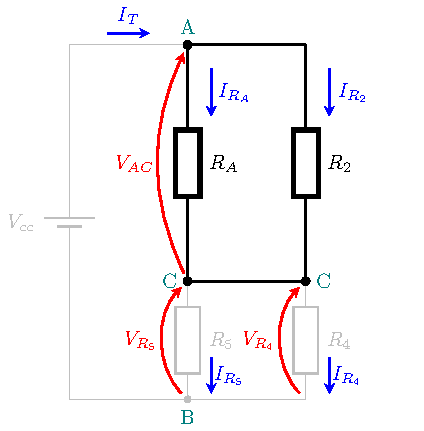
\includegraphics[scale=1.0]{fig-desafioPassoA}
    \end{figure}
  \end{minipage}
\end{minipage}








\subsection{Passo 11: Divisão da tensão}

\begin{minipage}{\linewidth}
  \centering
  \begin{minipage}{0.45\linewidth}
    Dados do circuito: \\
                $R_1 = 330\Omega$,
                $R_2 = 150\Omega$,
                $R_3 = 270\Omega$, \\
                $R_4 = 400\Omega$,
                $R_5 = 100\Omega$,
                $V_{CC} = 10V$, \\
                $R_A = R_1 + R_3 = 600\Omega$, \\
                $R_B = R_A // R_2 = 120\Omega$, \\
                $R_C = R_4 // R_5 = 80\Omega$, \\
                $R_T = R_B + R_C = 200\Omega$, \\
                \color{blue}
                $I_T = \frac{V_{AB}}{R_T} = 0,05 A$,\\
                \color{red}
                $V_{R_B} = \frac{R_B}{R_T} . V_{AB} = 6V$,\\
                $V_{R_C} = R_C.I_T = 4V$, \\
                $V_{R_C} = V_{CB} = V_{R_5} = V_{R_4}$,\\
                \color{blue}
                $I_{R_5} = V_{R_5} / R_5 = 0,04 A $, \\
                $I_{R_4} = V_{R_4} / R_4 = 0,01 A$, \\
                \color{red}
                $V_{R_B} = V_{AC} = V_{R_A} = V_{R_2}$, \\
                \color{blue}
                $I_{R_A} = V_{R_A} / R_A = 0,01 A$, \\
                $I_{R_2} = V_{R_2} / R_2 = 0,04 A$.
    \begin{eqnarray}
      I_{R_A} & = & I_{R_1} = I_{R_3} = 0,01 A \nonumber
    \end{eqnarray}
    \color{red}
    \vspace{-10mm}
    \begin{eqnarray}
      V_{R_1} = R_1 . I_{R_1} & = & 330 . 0,01 = 3,3 V \nonumber\\
      \nonumber\\
      V_{R_3} = R_3 . I_{R_3} & = & 270 . 0,01 = 2,7 V \nonumber
    \end{eqnarray}
  \end{minipage}
  \hspace{0.05\linewidth}
  \begin{minipage}{0.45\linewidth}
    \begin{figure}[H]
      \centering
      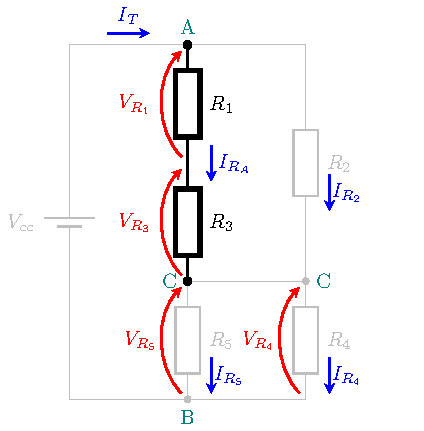
\includegraphics[scale=1.0]{fig-desafioPassoB}
    \end{figure}
  \end{minipage}
\end{minipage}







\subsection{Passo 12: Resultado }

\begin{minipage}{\linewidth}
  \centering
  \begin{minipage}{0.45\linewidth}
    Dados do circuito: \\
                $R_1 = 330\Omega$,
                $R_2 = 150\Omega$,
                $R_3 = 270\Omega$, \\
                $R_4 = 400\Omega$,
                $R_5 = 100\Omega$,
                $V_{CC} = 10V$, \\
                $R_A = R_1 + R_3 = 600\Omega$, \\
                $R_B = R_A // R_2 = 120\Omega$, \\
                $R_C = R_4 // R_5 = 80\Omega$, \\
                $R_T = R_B + R_C = 200\Omega$, \\
                \color{blue}
                $I_T = \frac{V_{AB}}{R_T} = 0,05 A$,\\
                \color{red}
                $V_{R_B} = \frac{R_B}{R_T} . V_{AB} = 6V$,\\
                $V_{R_C} = R_C.I_T = 4V$, \\
                $V_{R_C} = V_{CB} = V_{R_5} = V_{R_4}$,\\
                \color{blue}
                $I_{R_5} = V_{R_5} / R_5 = 0,04 A $, \\
                $I_{R_4} = V_{R_4} / R_4 = 0,01 A$, \\
                \color{red}
                $V_{R_B} = V_{AC} = V_{R_A} = V_{R_2}$, \\
                \color{blue}
                $I_{R_A} = V_{R_A} / R_A = 0,01 A$, \\
                $I_{R_2} = V_{R_2} / R_2 = 0,04 A$, \\
                $I_{R_A} = I_{R_1} = I_{R_3} = 0,01 A$, \\
                \color{red}
                $V_{R_1} = R_1 . I_{R_1} = 3,3 V$, \\
                $V_{R_3} = R_3 . I_{R_3} = 2,7 V$.
  \end{minipage}
  \hspace{0.05\linewidth}
  \begin{minipage}{0.45\linewidth}
    \begin{figure}[H]
      \centering
      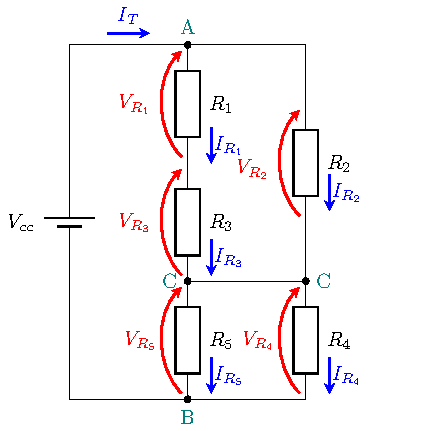
\includegraphics[scale=1.0]{fig-desafioPassoC}
    \end{figure}
  \end{minipage}
\end{minipage}
